\documentclass[10pt,a4paper]{article}
\usepackage[utf8]{inputenc}
\usepackage[T1]{fontenc}
\usepackage{lmodern}
\usepackage[margin=1.5cm, top=1.4cm, bottom=1.4cm]{geometry}
\usepackage{hyperref}
\usepackage{enumitem}
\usepackage{titlesec}
\usepackage{xcolor}
\usepackage{graphicx}

\definecolor{accent}{HTML}{00686E}
\hypersetup{colorlinks=true, urlcolor=accent, linkcolor=accent}
\pagenumbering{arabic}
\setlength{\parindent}{0pt}

\titleformat{\section}{\large\bfseries\color{accent}}{}{0em}{}[\vspace{-0.6em}\rule{\textwidth}{0.8pt}]
\titlespacing{\section}{0pt}{7pt}{4pt}

\newcommand{\role}[4]{%
  \textbf{#1} \hfill \textbf{#2}\\[1pt]%
  \textit{#3} \hfill \textit{#4}\\[2pt]%
}
\setlist[itemize]{leftmargin=1.2em, itemsep=1.5pt, topsep=2pt, parsep=0pt}

\begin{document}

% ================= HEADER =================
\begin{minipage}[c]{0.80\textwidth}
  {\Huge\bfseries Prabhavit Gupta}\\[3pt]
  {\color{accent}\large Senior Backend Systems Engineer: Distributed Pipelines, APIs \& Cloud Architecture}\\[6pt]
  {\footnotesize +39 351 610 7807 ~$\vert$~
  \href{mailto:prabhavitg@gmail.com}{prabhavitg@gmail.com} ~$\vert$~
  \href{https://www.linkedin.com/in/prabhavit/}{linkedin.com/in/prabhavit} ~$\vert$~
  \href{https://github.com/prab-gupta}{github.com/prab-gupta} ~$\vert$~
  Venice, Italy (CET Time Zone / EU Permanent Resident)}
\end{minipage}\hfill
\begin{minipage}[c]{0.18\textwidth}
  \raggedleft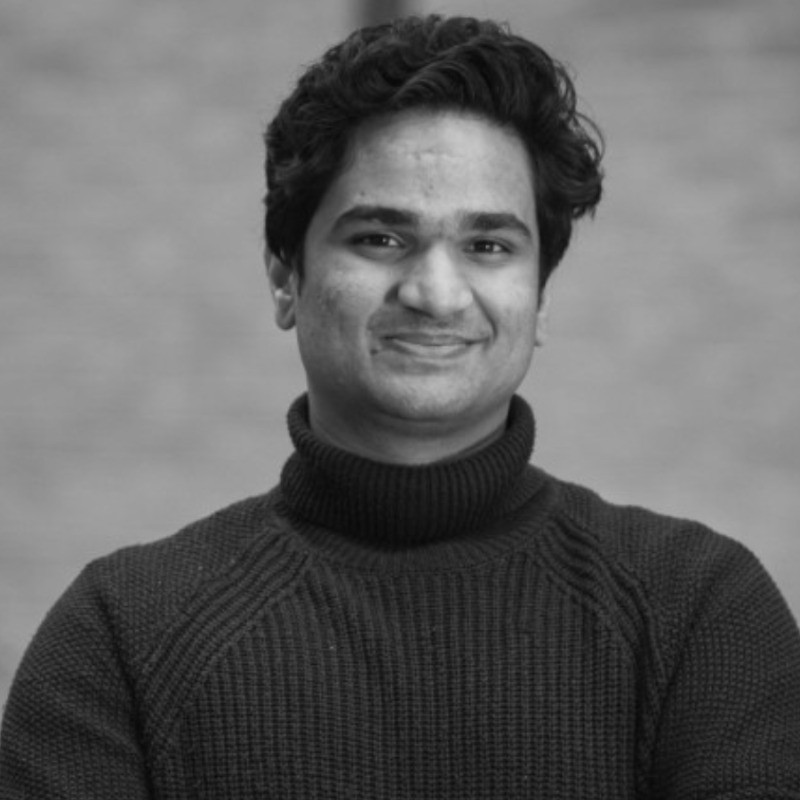
\includegraphics[width=2.0cm]{photo.jpg}
\end{minipage}
\vspace{-2pt}

% ================= SUMMARY =================
\section{Summary}
Senior Backend Systems Engineer with 3 years of commercial production experience designing, building, and operating high-throughput distributed backends, streaming data pipelines, and mission-critical cloud APIs. Proven track record architecting event-driven microservices that process millions of events daily with 99.8\% production reliability. Deep practical expertise across Python (FastAPI, asyncio), Node.js/TypeScript, PostgreSQL optimization, Redis message brokers, and containerized cloud architectures. Based in Venice, Italy (CET time zone) with an EU Long-Term Residence Permit (permanent unrestricted EU work authorization across all EU member states, no sponsorship required); available immediately for full-time remote roles.

% ================= TECHNICAL EXPERTISE =================
\section{Technical Expertise}
\begin{itemize}
  \item \textbf{Distributed Backend Systems:} High-throughput REST and asynchronous RPC APIs, event-driven microservice architectures, distributed task queues, rate-limiting, circuit breakers, and fault-tolerant service orchestration.
  \item \textbf{Data Pipelines \& Streaming:} Python (FastAPI, asyncio, pandas, NumPy, Pydantic), Node.js, real-time telemetry ingestion, ETL data processing, third-party messaging integrations, and webhook consumers.
  \item \textbf{Databases \& Caching:} PostgreSQL (advanced schema design, query optimization, indexing, ACID transactional boundaries), Redis (in-memory caching, pub/sub, atomic locking, queue management).
  \item \textbf{DevOps \& Infrastructure:} Docker containerization, cloud service architecture (AWS / GCP), GitHub Actions CI/CD automation, Prometheus/Grafana metric telemetry, structured JSON logging.
  \item \textbf{Applied AI \& Tooling:} Claude Code, Model Context Protocol (MCP) integrations, automated testing pipelines, and agentic workflows for accelerated system delivery.
  \item \textbf{Languages \& Authorization:} English (C1 Professional, fluent), Hindi (Native), Italian (Conversational). EU Long-Term Residence Permit (unrestricted EU work authorization across all EU member states, no sponsorship required).
\end{itemize}

% ================= EXPERIENCE =================
\section{Experience}

\role{\href{https://flowspace.co}{FlowSpace.co}}{Mar 2024 - Aug 2026}{Lead Backend \& AI Systems Engineer}{London, UK (remote)}
\begin{itemize}
  \item Architected and scaled high-throughput backend services powering an enterprise AI platform supporting 4,500+ active users across European organizations with 99.8\% uptime.
  \item Engineered asynchronous Python (FastAPI) and Node.js microservices handling real-time telemetry, automated data extraction, and high-concurrency client requests.
  \item Designed resilient database architectures in PostgreSQL and implemented distributed caching layers in Redis, reducing p95 database query latencies by 42\%.
  \item Integrated robust third-party APIs and webhook processors with idempotent delivery guarantees, automated retries, and comprehensive error auditing.
  \item Automated end-to-end integration test suites and multi-stage GitHub Actions CI/CD deployment pipelines, ensuring zero-downtime release rollouts.
\end{itemize}

\role{Urlink}{Apr 2025 - Jul 2025}{Backend Solutions Developer (Freelance)}{Barcelona, Spain (remote)}
\begin{itemize}
  \item Built scalable data ingestion microservices and RESTful API endpoints for external data synchronization across distributed enterprise platforms.
  \item Optimized PostgreSQL database queries and transactional boundaries, preventing data race conditions during high-volume ingestion cycles.
  \item Designed comprehensive API specifications and automated testing harnesses using Playwright and pytest to validate system contracts before client handover.
\end{itemize}

\role{Independent Technical Consultant}{Aug 2023 - Feb 2024}{Backend Systems \& Automation Developer}{Venice, Italy}
\begin{itemize}
  \item Engineered custom backend APIs, data pipelines, and asynchronous automation scripts using Python and TypeScript for European SMB clients.
  \item Implemented event-driven webhook listeners and database synchronization jobs, eliminating manual operational data entry.
  \item Produced detailed technical architecture documentation, database schema diagrams, and deployment runbooks for client operations.
\end{itemize}

% ================= EDUCATION =================
\section{Education}
\role{Ca' Foscari University of Venice}{2020 - 2024}{BA in Philosophy, International Studies and Economics}{Venice, Italy}
\begin{itemize}
  \item Rigorous foundational study in formal logic, epistemology, systems theory, and mathematical economic models.
\end{itemize}

\end{document}
